% !TeX root = ../../tesi.tex

For the acquisition of RGB-D data at Site~1, the \textbf{Microsoft Azure Kinect DK} \cite{microsoft_azure_nodate} was employed. This device is a spatial sensing platform developed by Microsoft, designed for advanced computer vision, depth sensing, and AI-based perception applications.

\begin{figure}[h]
    \centering
    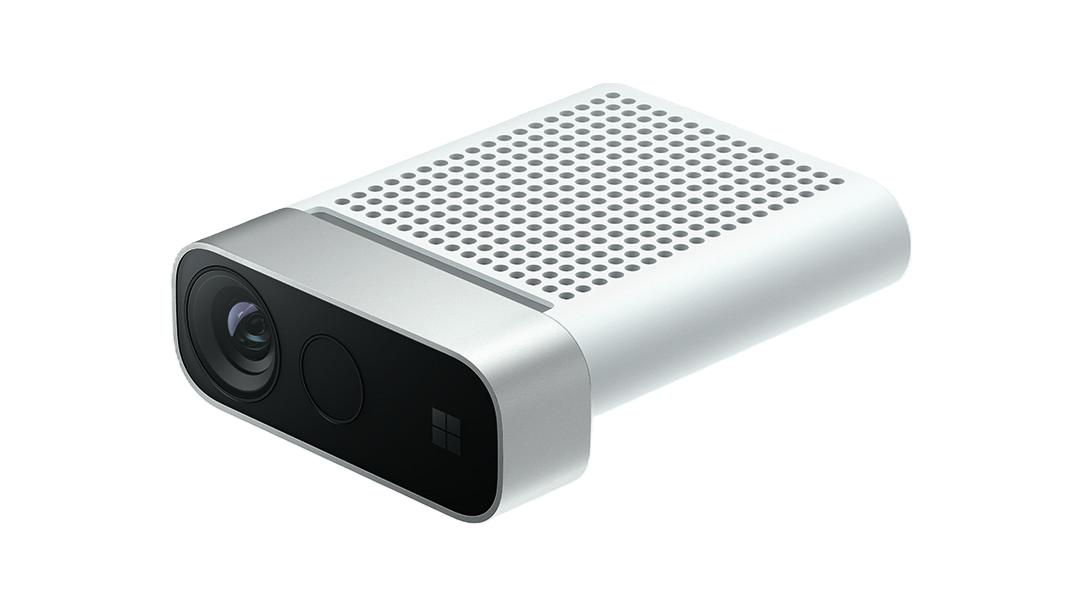
\includegraphics[width=0.6\linewidth]{images/azure-kinect.jpg}
    \caption{Microsoft Azure Kinect DK}
    \label{fig:azure-kinect}
\end{figure}

The Azure Kinect DK integrates a high-resolution RGB camera and a depth sensor based on Time-of-Flight (ToF) technology. The RGB camera provides up to 12~MP resolution (4096$\times$3072), while the depth sensor delivers depth maps with a maximum resolution of 1024$\times$1024 pixels.

The depth sensing module operates using modulated infrared light to estimate per-pixel distance information, enabling accurate 3D scene reconstruction \cite{microsoft_about_nodate}.

The device supports multiple depth operating modes, including Narrow Field of View (NFOV) and Wide Field of View (WFOV), each configurable with binned and unbinned resolutions, as illustrated in Figure~\ref{fig:camera-fov} and in Table~\ref{tab:azure_depth_modes}. This flexibility allows adaptation to different working distances and spatial accuracy requirements. The depth measurement range typically varies between 0.25~m and 5.5~m, depending on the selected configuration and environmental conditions \cite{microsoft_about_nodate}.

\begin{figure}[h]
    \centering
    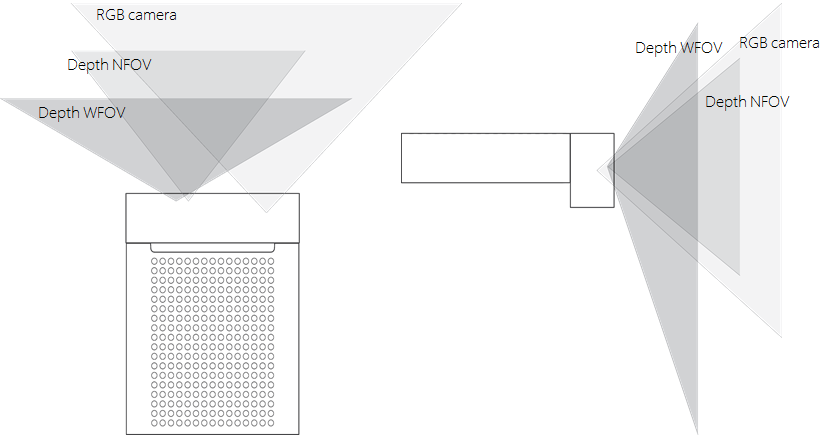
\includegraphics[width=0.70\linewidth]{images/camera-fov.png}
    \caption{Available depth sensor fields of view (NFOV and WFOV).}
    \label{fig:camera-fov}
\end{figure}

\newpage
Depending on the selected RGB resolution and depth operating mode, the camera parameters, field of view, frame rate, and operational range vary significantly. \\The main RGB camera configurations are reported in Table~\ref{tab:azure_rgb_modes}, while the available depth modes are summarized in Table~\ref{tab:azure_depth_modes}.

\begin{table}[h]
    \centering
    \renewcommand{\arraystretch}{1.2}
    \resizebox{\textwidth}{!}{
    \begin{tabular}{|l|c|l|c|c|}
        \hline
        \textbf{RGB Resolution (HxV)} & \textbf{Aspect Ratio} & \textbf{Format} & \textbf{FPS} & \textbf{Nominal FoV (HxV)} \\
        \hline
        3840$\times$2160 & 16:9 & MJPEG & 0, 5, 15, 30 & 90$^\circ$$\times$59$^\circ$ \\
        2560$\times$1440 & 16:9 & MJPEG & 0, 5, 15, 30 & 90$^\circ$$\times$59$^\circ$ \\
        1920$\times$1080 & 16:9 & MJPEG & 0, 5, 15, 30 & 90$^\circ$$\times$59$^\circ$ \\
        1280$\times$720  & 16:9 & MJPEG / YUY2 / NV12 & 0, 5, 15, 30 & 90$^\circ$$\times$59$^\circ$ \\
        4096$\times$3072 & 4:3  & MJPEG & 0, 5, 15 & 90$^\circ$$\times$74.3$^\circ$ \\
        2048$\times$1536 & 4:3  & MJPEG & 0, 5, 15, 30 & 90$^\circ$$\times$74.3$^\circ$ \\
        \hline
    \end{tabular}
    }
    \caption{RGB camera operating modes and specifications.}
    \label{tab:azure_rgb_modes}
\end{table}

\begin{table}[h]
    \centering
    \small
    \renewcommand{\arraystretch}{1.2}
    \begin{tabular}{|l|c|c|c|c|c|}
        \hline
        \textbf{Mode} & \textbf{Resolution} & \textbf{FoV} & \textbf{FPS} & \textbf{Operating Range} & \textbf{Exposure Time} \\
        \hline
        NFOV unbinned & 640$\times$576 & 75$\times$65$^\circ$ & 0, 5, 15, 30 & 0.5 -- 3.86 m & 12.8 ms \\
        NFOV 2$\times$2 binned & 320$\times$288 & 75$\times$65$^\circ$ & 0, 5, 15, 30 & 0.5 -- 5.46 m & 12.8 ms \\
        WFOV 2$\times$2 binned & 512$\times$512 & 120$\times$120$^\circ$ & 0, 5, 15, 30 & 0.25 -- 2.88 m & 12.8 ms \\
        WFOV unbinned & 1024$\times$1024 & 120$\times$120$^\circ$ & 0, 5, 15 & 0.25 -- 2.21 m & 20.3 ms \\
        Passive IR & 1024$\times$1024 & N/A & 0, 5, 15, 30 & N/A & 1.6 ms \\
        \hline
    \end{tabular}
    \caption{Depth camera operating modes and specifications.}
\label{tab:azure_depth_modes}
\end{table}
From a hardware standpoint, the Azure Kinect DK includes:
\begin{itemize}
    \item one 12~MP RGB camera,
    \item one Time-of-Flight depth sensor,
    \item one 6-axis inertial measurement unit (IMU),
    \item one USB-C interface for power and data transmission,
    \item one external synchronization port for multi-device configurations.
\end{itemize}

\begin{figure}[h]
    \centering
    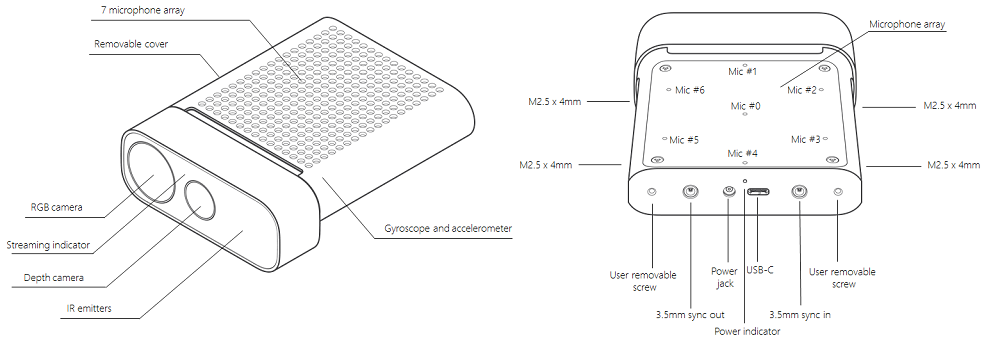
\includegraphics[width=0.8\linewidth]{images/kinect.png}
    \caption{Microsoft Azure Kinect DK hardware and connectivity.}
    \label{fig:kinect}
\end{figure}

The availability of synchronized RGB and depth streams enables the generation of geometrically aligned RGB-D frames, which are particularly suitable for 3D reconstruction, volumetric estimation, and point cloud generation. In the present application, depth information is exploited to estimate the volume of dough samples by reconstructing their three-dimensional point-cloud.

\subsubsection{Time-of-Flight Depth Sensing Principle}
% !TeX root = ../../tesi.tex

The depth sensing module of the Microsoft Azure Kinect DK is based on the Time-of-Flight (ToF) principle, a technique used to estimate the distance between the sensor and objects in the scene by measuring the time required for emitted light to travel to the target and back to the sensor.
\begin{figure}[h]
    \centering
    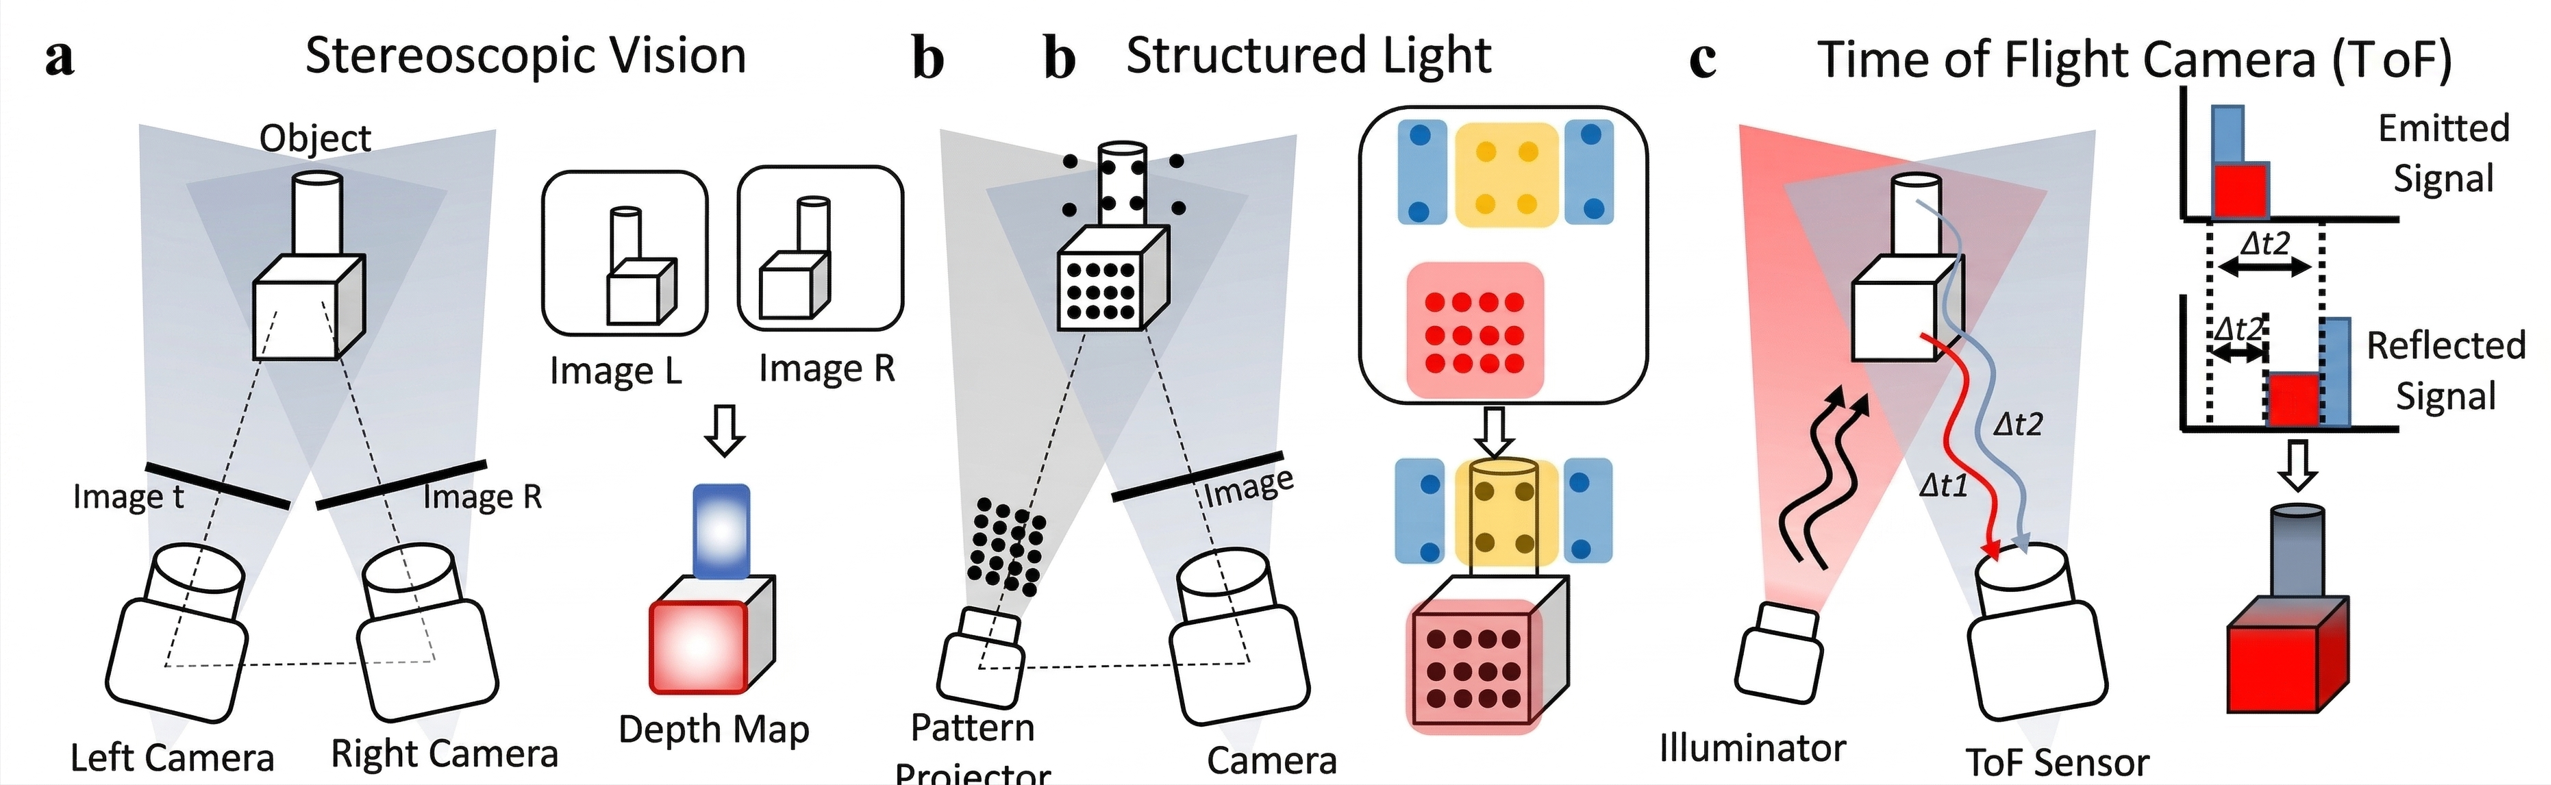
\includegraphics[width=0.7\linewidth]{images/ToF.png}
    \caption{Different depth estimation approaches}
    \label{fig:Depth}
\end{figure}

In general, the depth $Z$ of a point can be computed as:

\begin{equation}
Z = \frac{c \cdot \Delta t}{2}
\end{equation}

where:
\begin{itemize}
    \item $c$ is the speed of light in air,
    \item $\Delta t$ is the round-trip travel time of the emitted optical signal.
    \item The division by two accounts for the two-way propagation path (sensor-to-object and object-to-sensor).
\end{itemize}

Direct measurement of $\Delta t$ requires extremely high temporal resolution, as light travels approximately 30~cm in 1~ns. For this reason, most modern ToF cameras, including the Azure Kinect, employ a \textit{continuous-wave modulation} approach rather than direct pulsed time measurement.

\begin{figure}[h]
    \centering
    \includegraphics[width=0.5\linewidth]{images/ToF_pulse_vs_cont.jpg}
    \caption{Different ToF approaches}
    \label{fig:ToF_1}
\end{figure}

In continuous-wave ToF systems, the emitted infrared light is amplitude-modulated at a known frequency. The reflected signal received by the sensor exhibits a phase shift $\phi$ proportional to the propagation delay. The depth is then computed as:

\begin{equation}
Z = \frac{c}{4\pi f} \phi
\end{equation}

where:
\begin{itemize}
    \item $f$ is the modulation frequency,
    \item $\phi$ is the measured phase difference between emitted and received signals.
\end{itemize}

\begin{figure}[h]
    \centering
    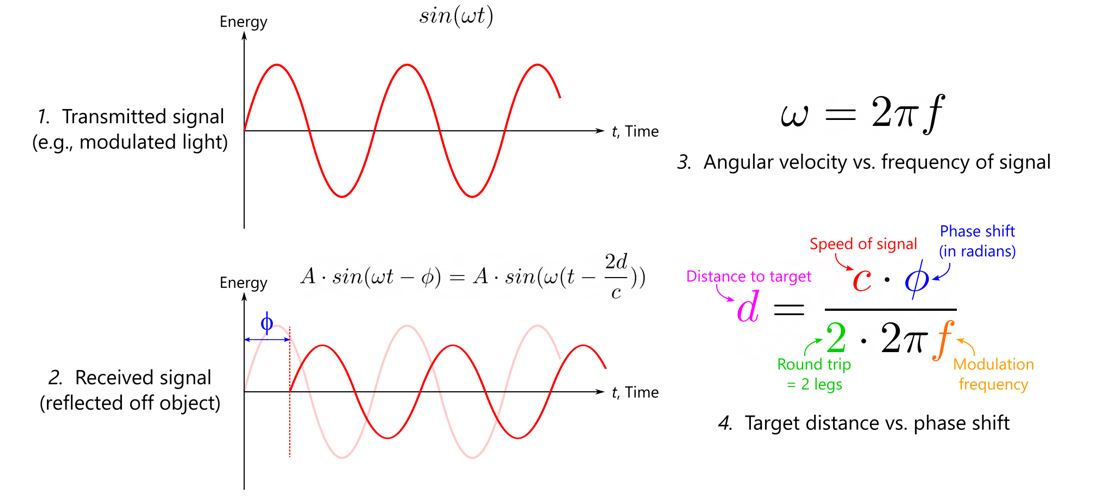
\includegraphics[width=0.7\linewidth]{images/ToF_1.jpg}
    \caption{Time of flight equations derivation}
    \label{fig:ToF_2}
\end{figure}

By estimating the phase shift at each pixel, the sensor generates a dense depth map, enabling per-pixel 3D reconstruction of the observed scene.
\\
The advantages of ToF-based depth sensing include:
\begin{itemize}
    \item direct acquisition of metric depth measurements,
    \item dense depth maps without requiring stereo matching,
    \item robustness to moderate textureless surfaces.
\end{itemize}

However, ToF systems are subject to several sources of error, including:
\begin{itemize}
    \item multipath interference (MPI), caused by indirect reflections,
    \item ambient infrared light interference,
    \item phase ambiguity at larger distances due to periodic modulation,
    \item reduced accuracy on highly reflective or absorptive materials.
\end{itemize}

Despite these limitations, Time-of-Flight technology provides accurate and dense depth measurements in indoor environments, making it particularly suitable for volumetric estimation and 3D reconstruction tasks, as required in the present application.


\subsubsection{Azure Kinect Sensor SDK}

The Azure Kinect DK is supported by the Azure Kinect Sensor SDK \cite{microsoft_azure-kinect-sensor-sdk_2026}, which provides low-level APIs for device control, stream acquisition, intrinsic and extrinsic calibration handling, depth-to-color transformation, and point cloud extraction \cite{microsoft_about_nodate}.

The SDK exposes calibrated camera parameters, including focal lengths, principal points, and distortion coefficients, enabling accurate geometric transformations between RGB and depth coordinate systems. Moreover, built-in functions allow real-time depth image rectification, coordinate mapping, and conversion of depth frames into 3D point clouds expressed in camera reference coordinates.

Such capabilities are particularly relevant in volumetric estimation tasks, where precise spatial alignment between depth measurements and RGB data is required to ensure geometrical consistency.
\begin{figure}[h]
    \centering
    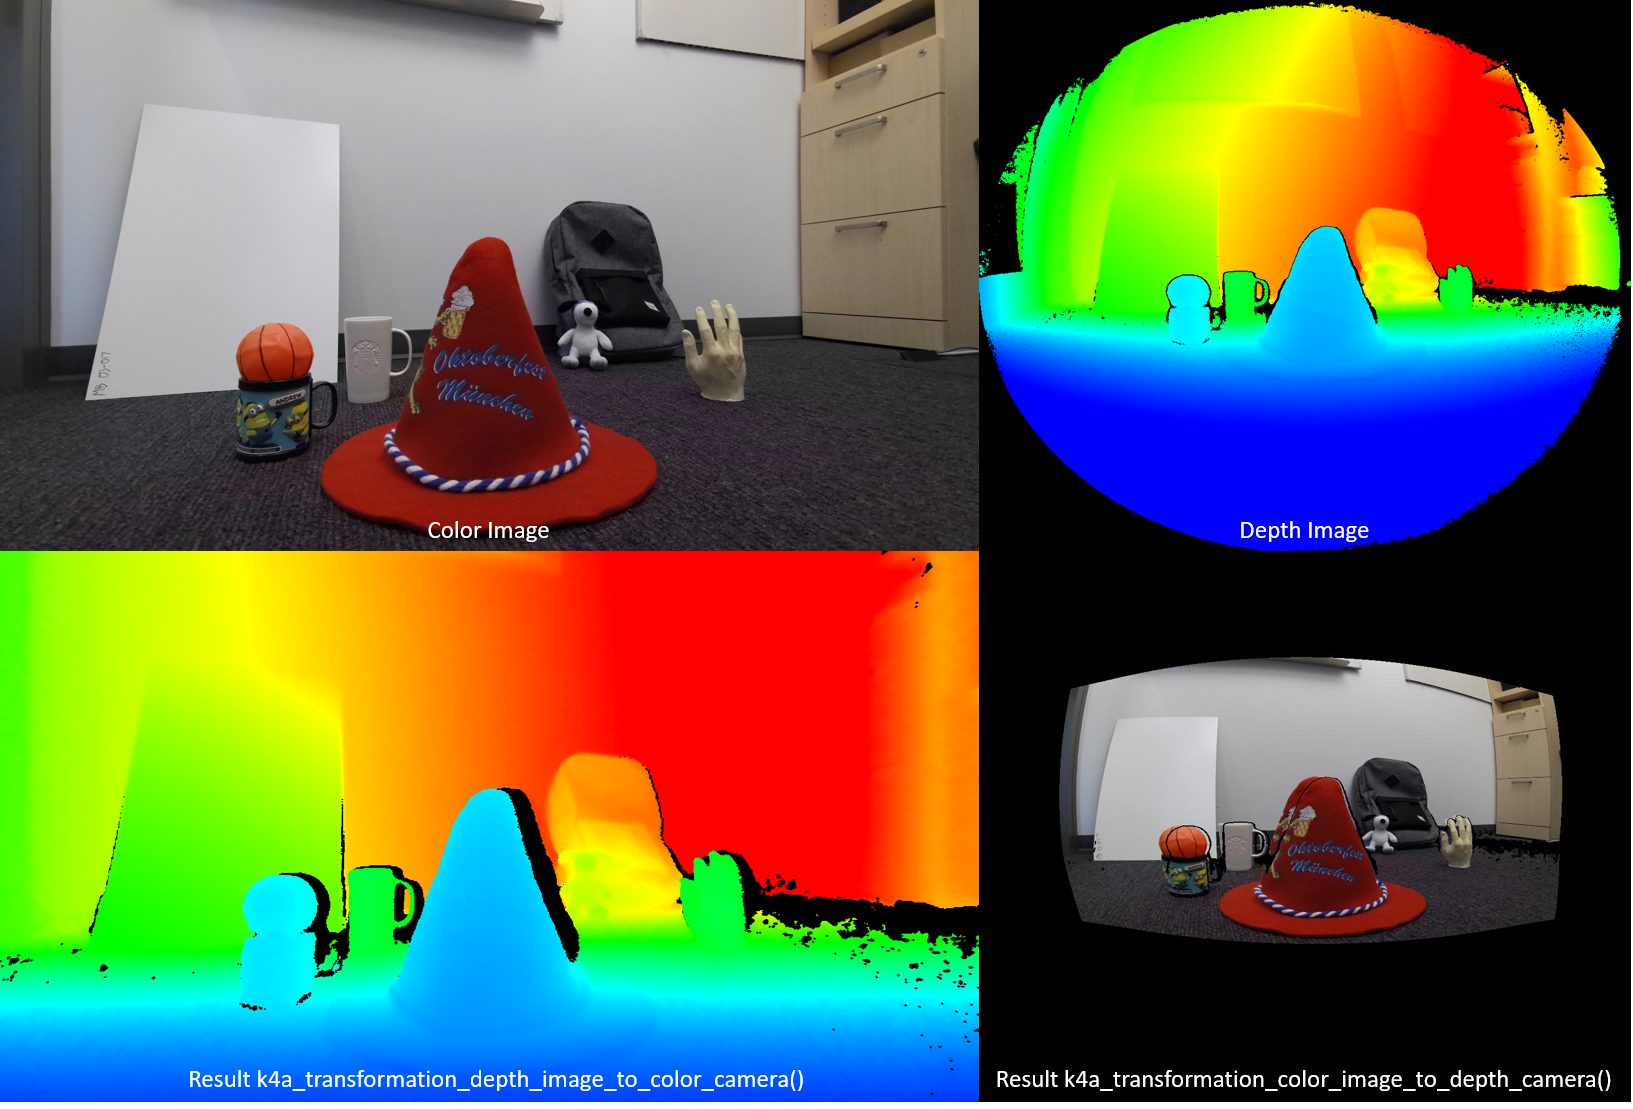
\includegraphics[width=0.5\linewidth]{images/sdk.png}
    \caption{Example of SDK transformation from depth image to color camera FOV and viceversa}
    \label{fig:SDK}
\end{figure}

\subsubsection{Python Wrapper: pyKinectAzure}
For integration within the data processing pipeline, a Python interface was adopted through the \textit{pyKinectAzure} wrapper \cite{gorordo_fernandez_pykinectazure_2026}. This open-source library provides Python bindings to the native Azure Kinect Sensor SDK, allowing device initialization, stream acquisition, frame synchronization, and calibration access directly from Python environments.

The wrapper enables rapid prototyping and seamless integration with scientific computing libraries such as NumPy and OpenCV. Through pyKinectAzure, depth frames can be converted into NumPy arrays, facilitating further processing steps such as filtering, segmentation, and 3D point cloud generation within the same software ecosystem used for machine learning and computer vision tasks.

The use of a Python wrapper significantly simplifies the development workflow while maintaining access to the underlying calibrated sensor data and geometric transformation utilities provided by the official SDK.

Considering its depth accuracy, configurable field of view, synchronized RGB-D acquisition capabilities, and extensive software support, the Microsoft Azure Kinect DK represents a suitable sensing solution for industrial computer vision applications requiring reliable volumetric measurements.
